\newpage
\section{Washing Composite State}

\subsection{Mathematical Representation}

\noindent As \textit{Washing} is a composite state, it is defined as the tuple $S = (Q, \Sigma_1, \Sigma_2, q_0, V, \Lambda)$, where\\

\noindent $Q = \{Monitoring, Warming~Up, Long~Cycle, Short~Cycle\}$\\
\noindent $\Sigma_1 = \{after(2mins), after(30mins), after(10mins)\}$\\
\noindent $\Sigma_2 = \emptyset$\\
\noindent $q_0: Monitoring$\\
\noindent $V: currentWaterTemperature, desiredWaterTemperature: \mathbb{R} \\
\indent cycle = \{short, long\}$\\
\noindent $\Lambda$: Transition specifications\\
\indent 1. $\rightarrow Monitoring$\\
\indent 2. $Monitoring \xrightarrow {\text {[currentWaterTemperature $\neq$ desiredWaterTemperature]}} Warming~Up$\\
\indent 3. $Monitoring \xrightarrow {\text {[currentWaterTemperature $\approx$ desiredWaterTemperature AND cycle is long]}} Long~Cycle$\\
\indent 4. $Monitoring \xrightarrow {\text {[currentWaterTemperature $\approx$ desiredWaterTemperature AND cycle is short]}} Short~Cycle$\\
\indent 5. $Warming~Up \xrightarrow {\text {after(2 mins)}} Monitoring$\\
\indent 6. $Short~Cycle \xrightarrow {\text {after(10 mins)}} Exit$\\
\indent 7. $Long~Cycle \xrightarrow {\text {after (30 mins)}} Exit$\\

\noindent The UML state diagram is shown in Figure~\ref{fig:Washing}.

\newpage

\subsection{State transition diagram}

\begin{figure}[h!]
	\centering
		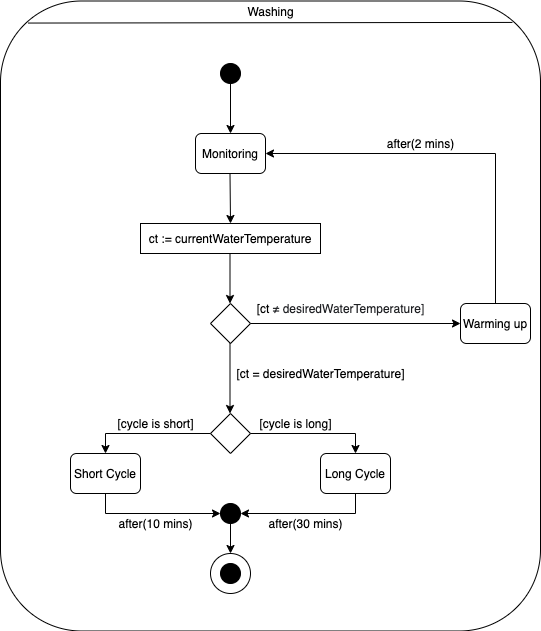
\includegraphics[width=0.8\textwidth]{Washing}
		  \caption{Washing State Diagram}
  \label{fig:Washing}
\end{figure}
